\textit{I dette kapitel designes, implementeres og testes hver blok af det samlede system og afslutningsvist testes hele systemet samlet. Det sikres herved, at hver del overholder kravspecifikationerne og derved teoretisk burde fungere sammen når systemet sammensættes.}

Systemet er opbygget af forskellige blokke, hvor designes og testes individuelt, hvor de efterfølgende vil blive samlet og testet. Disse blokke designes med henblik på at sikre systemets funktionalitet, hvorfor de designes ud fra kravspecifikationen.

\begin{figure}[H]
	\centering
	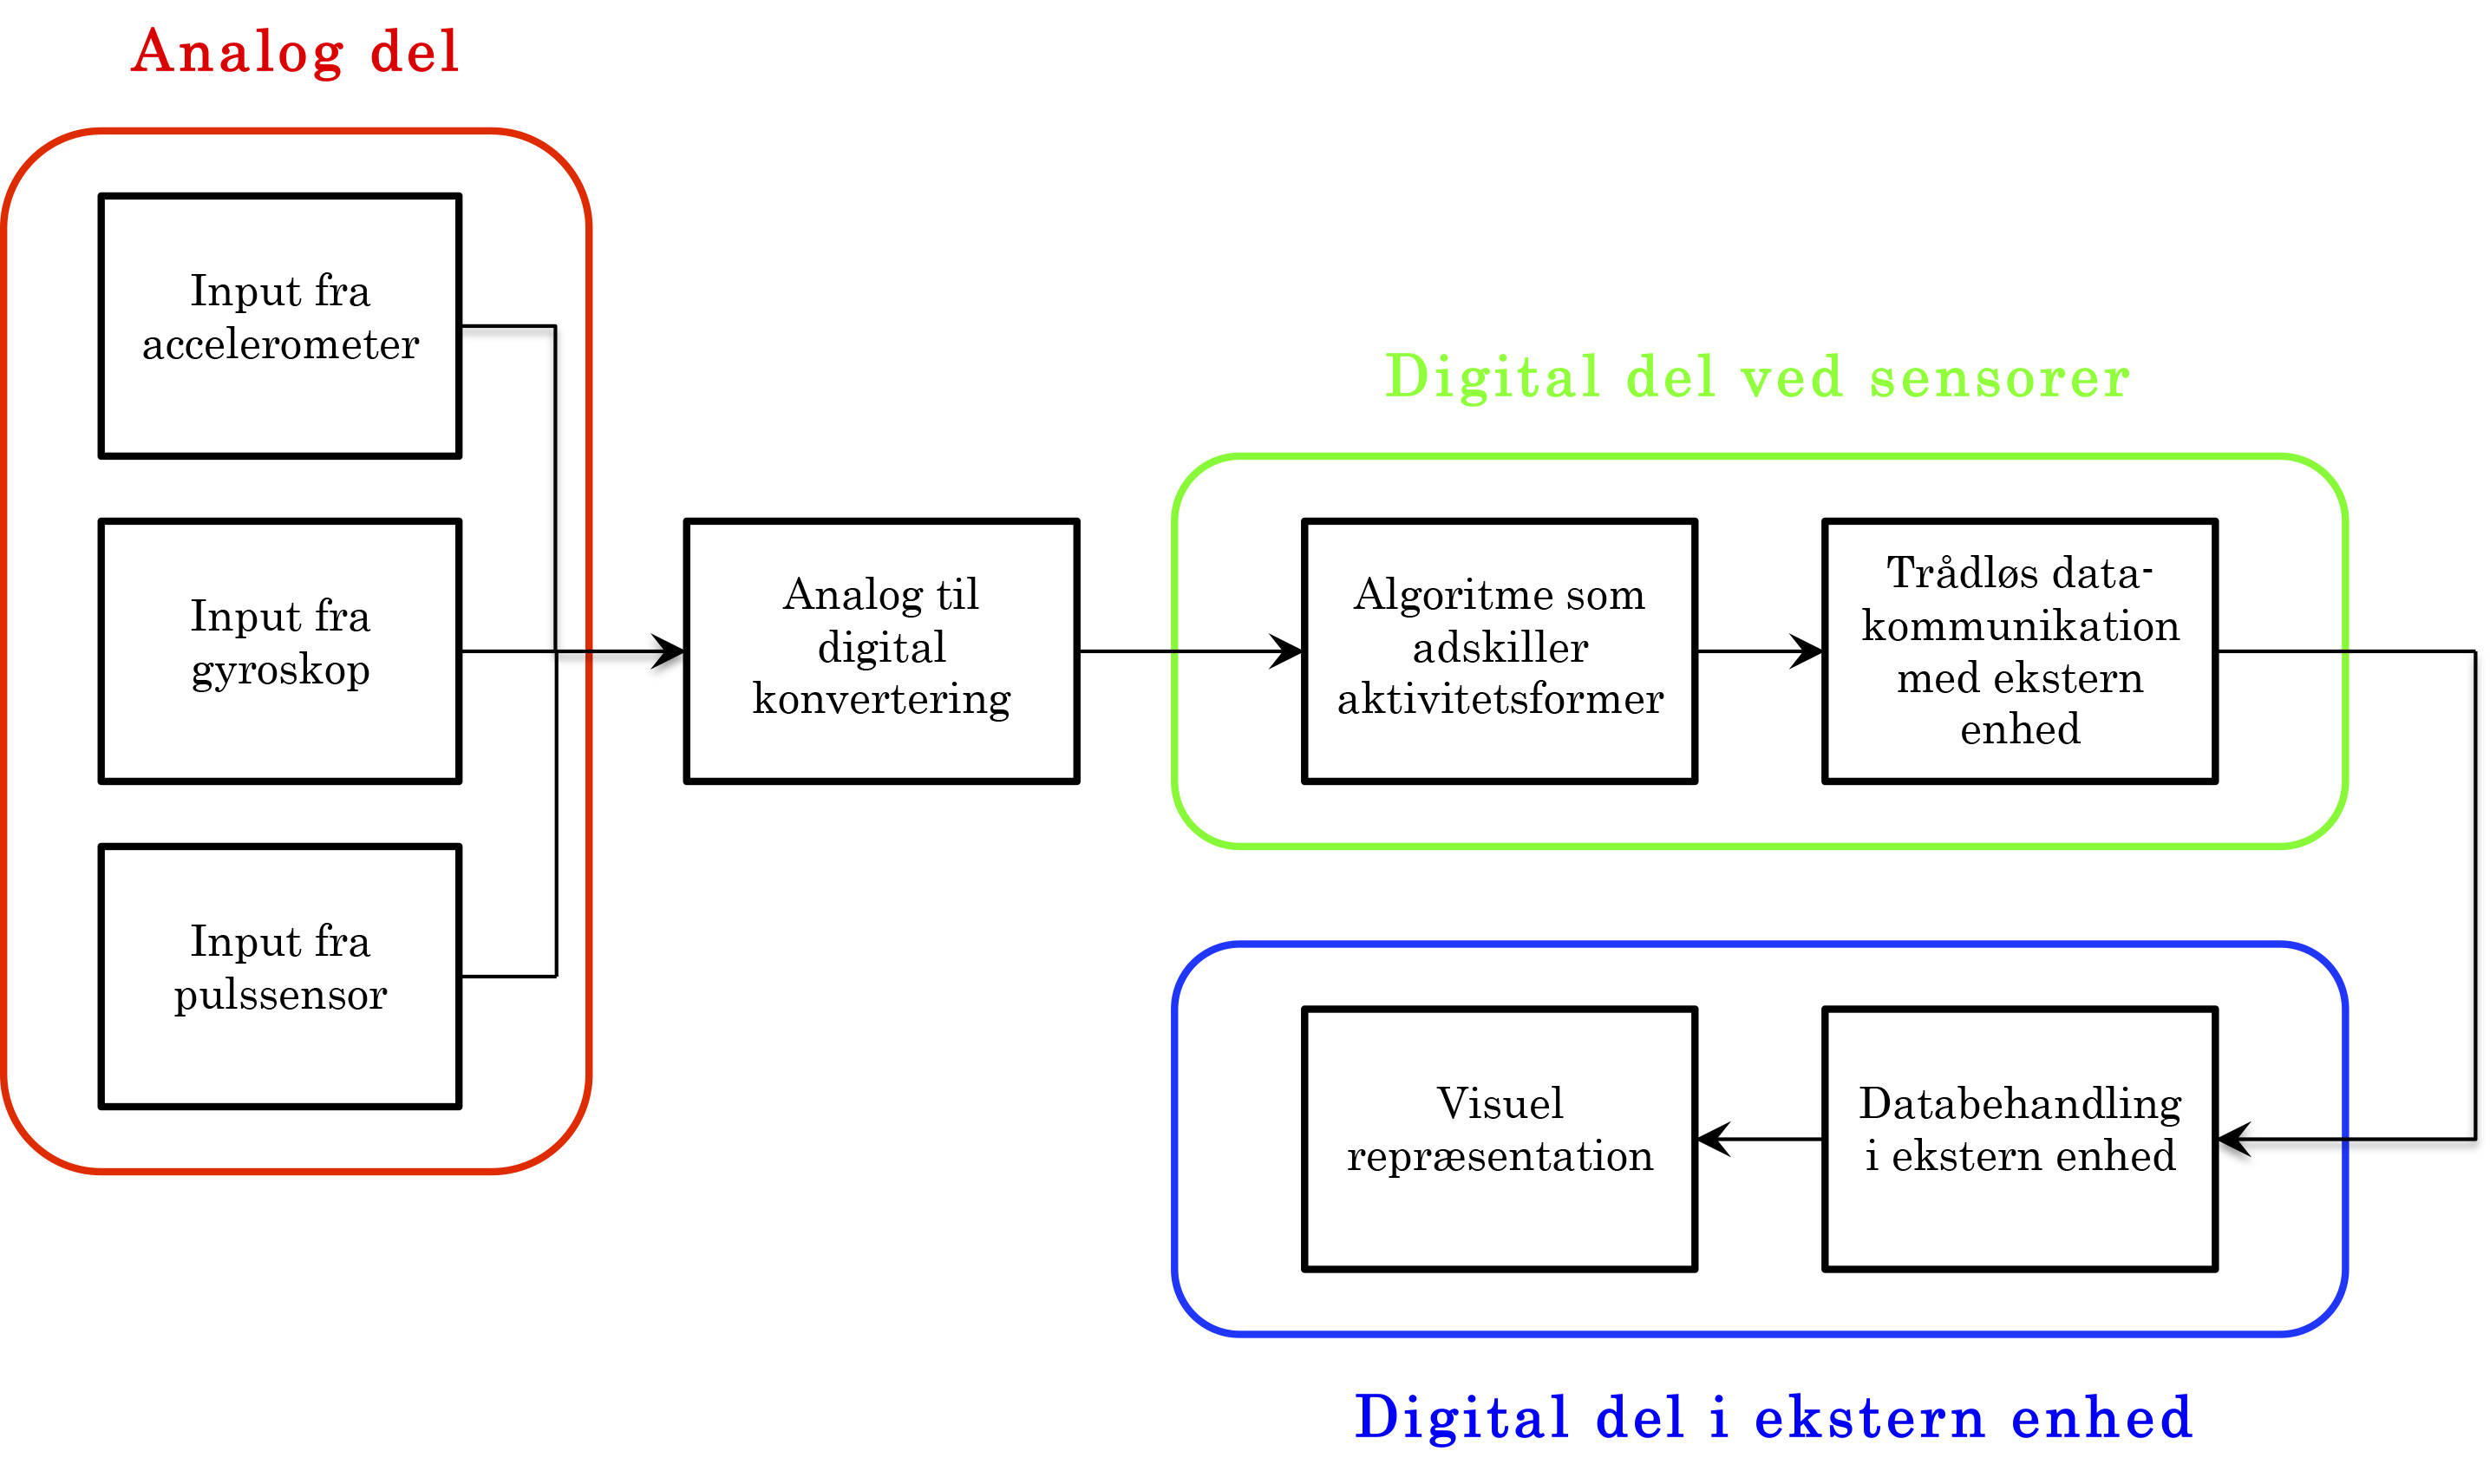
\includegraphics[scale=0.45]{figures/bProblemloesning/blokdiagram.png}
	\caption{På figuren ses blokdiagram for det samlede system, hvor et input modtages fra brugeren gennem sensorer, hvilket behandles i en GAP peripheral MCU. Herefter sendes dataet via BLE til en computer gennem en GAP central MCU, hvor det visualiseres på en brugerflade.}
	\label{fig:design_blokdiagram}
\end{figure}

Blokkene implementeres forskellige stedet i det samlede system, som vist på \figref{fig:design_blokdiagram}, hvoraf spændingsforsyning tilkobles GAP peripheral MCUen, hvor sensorer også tilkobles. På denne MCU vil signalerne blive digitaliseret og algoritmer vil efterfølgende behandle og adskille aktiviteterne gang, løb og cykling, samt udregne en tilhørende puls. Disse data sendes via BLE til en GAP central MCU som er koblet til en computer. På computeren vil dataet blive visualiseret igennem en MATLAB GUI, hvor brugeren kan følge sin progression.\fxnote{Vil vi have denne tekst før eller efter billedet?}  